\documentclass{beamer}
\usepackage[utf8]{inputenc}
\usepackage[T1]{fontenc}
% \usepackage{amscd, amsfonts, amsmath, amssymb, amstext, amsthm, caption, epsfig, fancyhdr, float, graphicx, latexsym, mathtools, multicol, multirow, algorithm, chngcntr}
\usepackage[english, french]{babel}
\usepackage{booktabs}

\usepackage{amsmath,amssymb}
\usepackage{graphicx}
\usepackage{caption}
\usepackage{subfig}
\usepackage{xspace}
\usepackage{fourier}

\usepackage{algorithm}
% \usepackage{algorithmic}
\usepackage{algorithmicx}
\usepackage{listings}
\usepackage{algcompatible}
\usepackage{algpseudocode} 

\usepackage{tikz}
\usetikzlibrary{shapes,arrows}
\usepackage{tkz-graph}
\usetikzlibrary{automata,arrows,positioning,calc}
\usetikzlibrary{positioning}
\usetikzlibrary{fit}
\usetikzlibrary{backgrounds}
\usetikzlibrary{calc}
\usetikzlibrary{shapes}
\usetikzlibrary{mindmap}
\usetikzlibrary{decorations.text}
\usetikzlibrary{snakes}

% \theoremstyle{definition} % insert bellow all blocks you want in normal text
% \newtheorem{definition}{Definition}



% tikzmark command, for shading over items
\newcommand{\tikzmark}[1]{\tikz[overlay,remember picture] \node (#1) {};}
% Define block styles
\tikzstyle{decision} = [diamond, draw, fill=blue!20,
    text width=4.5em, text badly centered, node distance=3cm, inner sep=0pt]
\tikzstyle{block} = [rectangle, draw, fill=blue!20,
    text width=5em, text centered, rounded corners]
\tikzstyle{line} = [draw]
\tikzstyle{cloud} = [draw, ellipse,fill=red!20, node distance=3cm,
    minimum height=2em]

\usepackage[most]{tcolorbox}

\setbeamertemplate{blocks}[rounded][shadow=true] % use rounded blocks with standard beamer shadow


% Distributions.
\newcommand*{\UnifDist}{\mathsf{Unif}}
\newcommand*{\ExpDist}{\mathsf{Exp}}
\newcommand*{\DepExpDist}{\mathsf{DepExp}}
\newcommand*{\GammaDist}{\mathsf{Gamma}}
\newcommand*{\LognormalDist}{\mathsf{LogNorm}}
\newcommand*{\WeibullDist}{\mathsf{Weib}}
\newcommand*{\ParetoDist}{\mathsf{Par}}
\newcommand*{\NormalDist}{\mathsf{Norm}}

\newcommand*{\GeometricDist}{\mathsf{Geom}}
\newcommand*{\NegBinomialDist}{\mathsf{NegBin}}
\newcommand*{\PoissonDist}{\mathsf{Poisson}}
\newcommand*{\BivariatePoissonDist}{\mathsf{BPoisson}}
\newcommand*{\CyclicalPoissonDist}{\mathsf{CPoisson}}

\newcommand*{\iid}{\textbf{iid}\@\xspace}
\newcommand*{\pdf}{\textbf{pdf}\@\xspace}
\newcommand*{\cdf}{\textbf{cdf}\@\xspace}
\newcommand*{\pmf}{\textbf{pmf}\@\xspace}
\newcommand*{\abc}{{\textbf{abc}}\@\xspace}
\newcommand*{\smc}{\textbf{smc}\@\xspace}
\newcommand*{\mcmc}{\textbf{mcmc}\@\xspace}
\newcommand*{\ess}{\textbf{ess}\@\xspace}
\newcommand*{\mle}{\textbf{mle}\@\xspace}
\newcommand*{\bic}{\textbf{bic}\@\xspace}
\newcommand*{\kde}{\textbf{kde}\@\xspace}
\newcommand*{\glm}{\textbf{glm}\@\xspace}
\newcommand*{\xol}{\textbf{xol}\@\xspace}
\newcommand*{\cpu}{\textbf{cpu}\@\xspace}
\newcommand*{\gpu}{\textbf{gpu}\@\xspace}
\newcommand*{\arm}{\textbf{arm}\@\xspace}

\def \si {\sigma}
\def \la {\lambda}
\def \al {\alpha}
% \def\e*{\end{eqnarray*}}
\def \di{\displaystyle}

\def \E{\mathbb E}
\def \N{\mathbb N}
\def \Z{\mathbb Z}
\def \NZ{\mathbb{N}_0}
\def \I{\mathbb I}
\def \w{\widehat}
\def \P {\mathbb P}
\def \V{\mathbb V}


\newcommand{\CL}{\mathbb{C}}
\newcommand{\RL}{\mathbb{R}}
\newcommand{\nat}{{\mathbb N}}
\newcommand{\Laplace}{\mathscr{L}}
\newcommand{\e}{\mathrm{e}}
\newcommand{\ve}{\bm{\mathrm{e}}} % vector e

\renewcommand{\L}{\mathcal{L}} % e.g. L^2 loss.

\newcommand{\ih}{\mathrm{i}}
\newcommand{\oh}{{\mathrm{o}}}
\newcommand{\Oh}{{\mathcal{O}}}
\newcommand{\Exp}{\mathbb{E}}

\newcommand{\Norm}{\mathcal{N}}
\newcommand{\LN}{\mathcal{LN}}
\newcommand{\SLN}{\mathcal{SLN}}

\renewcommand{\Pr}{\mathbb{P}}
\newcommand{\Ind}{\mathbb I}
\newcommand\bfsigma{\bm{\sigma}}
\newcommand\bfSigma{\bm{\Sigma}}
\newcommand\bfLambda{\bm{\Lambda}}
\newcommand{\stimes}{{\times}}
\def \limsup{\underset{n\rightarrow+\infty}{\overline{\lim}}}
\def \liminf{\underset{n\rightarrow+\infty}{\underline{\lim}}}




% vertical separator macro
\newcommand{\vsep}{
  \column{0.0\textwidth}
    \begin{tikzpicture}
      \draw[very thick,black!10] (0,0) -- (0,7.3);
    \end{tikzpicture}
}
\newcommand\blfootnote[1]{%
  \begingroup
  \renewcommand\thefootnote{}\footnote{#1}%
  \addtocounter{footnote}{-1}%
  \endgroup
}

% More space between lines in align
% \setlength{\mathindent}{0pt}

% Beamer theme
\usetheme{ZMBZFMK}
\usefonttheme[onlysmall]{structurebold}
\mode<presentation>
\setbeamercovered{transparent=10}

% align spacing
\setlength{\jot}{0pt}

\setbeamertemplate{navigation symbols}{}%remove navigation symbols

\title[BLOCKASTICS I]{Stochastic Models for blockchain analysis}
\subtitle{Consensus protocols}
\author{Pierre-O. Goffard}
\institute[ISFA]{Institut de Science Financières et d'Assurances\\
 \texttt{pierre-olivier.goffard@univ-lyon1.fr}
}
\date{\today}
% \titlegraphic{\includegraphics[width=2.5cm]{../../../Figures/bfs_logo.png}} 

\begin{document}
\begin{frame}
  \titlepage
\end{frame}
\begin{frame}{Consensus protocol}
\begin{tcolorbox}[enhanced,drop shadow, title=Definition]
    Algorithm to allows the full nodes to agree on a common data history
\end{tcolorbox}
It must rely on the scarce resources of the network
\begin{itemize}
  \item bandwidth
  \item computational power
  \item storage (disk space)
\end{itemize}
\end{frame}
\begin{frame}{Types of consensus protocols}
\begin{enumerate}
  \item Voting based 
  \footnotesize
\begin{thebibliography}{1}

\bibitem{lamport1982the}
L.~Lamport, R.~Shostak, and M.~Pease, ``The byzantine generals problem,'' {\em
  ACM Transactions on Programming Languages and Systems}, pp.~382--401, July
  1982.

\end{thebibliography}
\normalsize
  \item Leader based
  \begin{itemize}
    \item Proof-of-Work (computational power)
    \item Proof-of-Capacity and Proof-of-Spacetime (storage)
    \item Proof-of-Interaction (bandwidth)
    \item Proof-of-Stake (tokens)
  \end{itemize}
\end{enumerate}
\end{frame}
\begin{frame}{Conflict resolution in blockchain}
\begin{tcolorbox}[enhanced,drop shadow, title=Fork]
    A fork arises when there is a disagreement between the nodes resulting in several branches in the blockchain.
\end{tcolorbox}
\begin{tcolorbox}[enhanced,drop shadow, title=LCR]
    The \textit{Longest Chain Rule} states that if there exist several branches of the blockchain then the longest should be trusted.
\end{tcolorbox}
In practice 
\begin{itemize}
  \item A branch can be considered legitimate if it is $k\in\mathbb{N}$ blocks ahead of its pursuers.
  \item Fork can be avoided when
  $$
  \text{block appending time}> \text{ propagation delay} 
  $$
\end{itemize}
\end{frame}
\begin{frame}{Two generals problem}
Two nodes who must agree are communicating through an unreliable link.
\begin{itemize}
  \item Analogy with two generals besieging a city
\end{itemize}
The generals exchange messages through enemy territory
\begin{itemize}
\item[G1]$$\texttt{"I will attack tomorrow at dawn, if you confirm"}$$
\item[G2] $$\texttt{"I will follow your lead, if you confirm"}$$
\end{itemize}
\begin{figure}[ht!]
 \begin{center}
\begin{tikzpicture}[->, >=stealth', auto, semithick, node distance=3cm]
\tikzstyle{every state}=[fill=white,draw=black,thick,text=black,scale=0.8]
\node[state]    (1)                     {$G_1$};
\node[state]    (2)[right of=1]   {$G_2$};
\path
(1) edge[bend left]     node{Attack}     (2)
(2) edge[bend left]     node{Confirmation}      (1);
\end{tikzpicture}
\end{center}
\caption{Message and confirmation loop}
\label{fig:message_loop}
\end{figure}
\end{frame}
\begin{frame}{Byzantine General problem}
    $n$ generals must agree on a common battle plan, to either 
    \begin{itemize}
    \item Attack (A) 
    \item Retreat (R)
  \end{itemize}
\begin{tcolorbox}[enhanced,drop shadow, title=Problem]
There are $m<n$ traitors among the generals
\end{tcolorbox}
\begin{enumerate}
\item message $m(i,j)$ is sent to general $j$ by general $i$ 
\item Consensus is reached as general $j$ applies 
$$
f(\{m(i,j);\text{ }i = 1,\ldots,n\}) = \begin{cases}
A,& \text{if }\sum_{i = 1}^n\mathbb{I}_{m(i,j) =A} >n/2,\\
R, &\text{else}.
\end{cases}
$$
\end{enumerate}
\end{frame}
\begin{frame}[plain]
\begin{figure}[!ht]
 \begin{center}
 \subfloat[No traitor]{
\begin{tikzpicture}[->, >=stealth', auto, semithick, node distance=2cm]
\tikzstyle{every state}=[fill=white,draw=black,thick,text=black,scale=0.8]
\node[state]    (1)                     {$G_1$};
\node[state]    (2)[below of=1]   {$G_2$};
\node[state]    (3)[below of=2]   {$G_3$};
\node[state]    (4)[below of=3]   {$G_4$};
\node[state]    (5)[below of=4]   {$G_5$};
\node[draw] (6) [right of=1]   { \footnotesize$f({A,R,R,A,A}) = A$};
\node[draw] (7) [right of=2]   { \footnotesize$f({A,R,R,A,A}) = A$};
\node[draw] (8) [right of=3]   { \footnotesize$f({A,R,R,A,A}) = A$};
\node[draw] (9) [right of=
4]   { \footnotesize$f({A,R,R,A,A}) = A$};
\node[draw] (10) [right of=5]   { \footnotesize$f({A,R,R,A,A}) = A$};
\path
(1) edge[bend left]     node{ A}     (2)
(2) edge[bend left]     node{ R}      (1)
(2) edge[bend left]     node{ R}      (3)
(3) edge[bend left]     node{ R}      (2)
(3) edge[bend left]     node{ R}      (4)
(4) edge[bend left]     node{ A}      (3)
(4) edge[bend left]     node{ A}      (5)
(5) edge[bend left]     node{ A}      (4)
;
\path
(1) edge     (6)
(2) edge     (7)
(3) edge     (8)
(4) edge     (9)
(5) edge     (10)
;
\end{tikzpicture}
\label{fig:no_traitor}}
\hskip2em
 \subfloat[One traitor]{
\begin{tikzpicture}[->, >=stealth', auto, semithick, node distance=2cm]
\tikzstyle{every state}=[fill=white,draw=black,thick,text=black,scale=0.8]
\node[state]    (1)                     {$G_1$};
\node[state]    (2)[below of=1]   {$G_2$};
\node[state]    (3)[below of=2]   {$G_3$};
\node[state]    (4)[below of=3]   {\color{red}$G_4$};
\node[state]    (5)[below of=4]   {$G_5$};
\node[draw] (6) [right of=1]   { \footnotesize$f({A,R,R,R,A}) = R$};
\node[draw] (7) [right of=2]   { \footnotesize$f({A,R,R,R,A}) = R$};
\node[draw] (8) [right of=3]   { \footnotesize$f({A,R,R,R,A}) = R$};
\node[draw] (9) [right of=
4]   { \footnotesize$f({A,R,R,?,A}) = ?$};
\node[draw] (10) [right of=5]   { \footnotesize$f({A,R,R,A,A}) = A$};
\path
(1) edge[bend left]     node{ A}     (2)
(2) edge[bend left]     node{ R}      (1)
(2) edge[bend left]     node{ R}      (3)
(3) edge[bend left]     node{ R}      (2)
(3) edge[bend left]     node{ R}      (4)
(4) edge[bend left]     node{ \color{red}R}      (3)
(4) edge[bend left]     node{ \color{red}A}      (5)
(5) edge[bend left]     node{ A}      (4)
;
\path
(1) edge     (6)
(2) edge     (7)
(3) edge     (8)
(4) edge     (9)
(5) edge     (10)
;
\end{tikzpicture}
\label{fig:_one_traitor}}
\end{center}
\caption{Majority vote with or without a traitor}
\label{fig:majority_vote}
\end{figure}
\end{frame}
\begin{frame}{Commanders and Lieutenants}
One general is the commander while the others are the lieutenants
\begin{tcolorbox}[enhanced,drop shadow, title=Objective]
Design an algorithm so that the following conditions are met:
\begin{itemize}
  \item[C1] All the loyal lieutenants obey the same order
  \item[C2] If the commanding general is loyal, then  every loyal lieutenants obey the order he sends
\end{itemize}
\end{tcolorbox}
\begin{tcolorbox}[enhanced,drop shadow, title=Byzantine Fault Tolerance Theorem (Lamport et al.)]
There are no solution to the Byzantine General problem for $n<3m+1$ generals, where $m$ is the number of traitors.
\end{tcolorbox}
\end{frame}
\begin{frame}[plain]
\begin{figure}[!ht]
 \begin{center}
 \subfloat[Commander is loyal]{
\begin{tikzpicture}[->, >=stealth', auto, semithick, node distance=4cm]
\tikzstyle{every state}=[fill=white,draw=black,thick,text=black,scale=0.8]
\node[state]    (1)               {C};
\node[state]    (2)[below left of=1]   {L1};
\node[state]    (3)[below right of=1]   {\begin{color}{red}L2 \end{color}};
\path
(1) edge[bend left]     node{A}     (3)
(1) edge[bend right, above]     node{A}      (2)
(2) edge[bend left]     node{A}      (3)
(3) edge[bend left]     node{R}      (2)
% (3) edge[bend left]     node{R}      (4)
% (4) edge[bend left]     node{A}      (3)
% (4) edge[bend left]     node{A}      (5)
% (5) edge[bend left]     node{A}      (4)
;
\end{tikzpicture}
\label{fig:commander_loyal}}
\hskip2em
\subfloat[Commander is a traitor]{
\begin{tikzpicture}[->, >=stealth', auto, semithick, node distance=4cm]
\tikzstyle{every state}=[fill=white,draw=black,thick,text=black,scale=0.8]
\node[state]    (1)               {\begin{color}{red}C \end{color}};
\node[state]    (2)[below left of=1]   {L1};
\node[state]    (3)[below right of=1]   {L2};
\path
(1) edge[bend left, above]     node{A}     (3)
(1) edge[bend right, above]     node{R}      (2)
(2) edge[bend left]     node{R}      (3)
(3) edge[bend left]     node{A}      (2)
% (3) edge[bend left]     node{R}      (4)
% (4) edge[bend left]     node{A}      (3)
% (4) edge[bend left]     node{A}      (5)
% (5) edge[bend left]     node{A}      (4)
;
\end{tikzpicture}
\label{fig:commander_traitor}}
\end{center}
\caption{Majority vote with or without a traitor}
\label{fig:majority_vote}
\end{figure}
\end{frame}
\begin{frame}[plain]
\begin{algorithm}[H]
\caption{The Oral message algorithm $\text{OM}(m)$}\label{alg:om}
\begin{algorithmic}
\If{$m=0$};
\For{$i =1 \to n-1$} 
\State Commander sends $v_i = v$ to lieutenant $i$ 
\State Lieutenant $i$ set their value to $v$
\EndFor
\EndIf
\If{$m>0$};
\For{$i =1 \to n-1$} 
\State Commander sends $v_i$ to lieutenant $i$ 
\State Lieutenant $i$ uses OM(m-1) to communicate $v_i$ to the $n-2$ lieutenants
\EndFor
\For{$i =1 \to n-1$} 
\State Lieutenant $i$ set their value to $f(v_1, \ldots, v_{n-1})$
\EndFor
\EndIf
\end{algorithmic}
\end{algorithm}
\end{frame}
\begin{frame}{$n = 4$ and $m = 1$: Step 1}
\begin{figure}[!ht]
 \begin{center}
 \subfloat[Commander is loyal]{
\begin{tikzpicture}[->, >=stealth', auto, semithick, node distance=4cm]
\tikzstyle{every state}=[fill=white,draw=black,thick,text=black,scale=0.8]
\node[state]    (1)               {C};
\node[state]    (2)[below left of=1]   {L1};
\node[state]    (3)[below of=1]   {L2};
\node[state]    (4)[below right of=1]   {\begin{color}{red}L3 \end{color}};
\path
(1) edge[bend right]     node{A}     (2)
(1) edge[bend left]     node{A}      (4)
(1) edge     node{A}      (3)
% (2) edge[bend right, below]     node{A}      (3)
% (3) edge[bend right, above]     node{A}      (2)
% (4) edge[bend right, above]     node{R}      (3)
% (3) edge[bend right, below]     node{A}      (4)
;
\end{tikzpicture}
\label{fig:commander_loyal_om}}
\hskip2em
\subfloat[Commander is a traitor]{
\begin{tikzpicture}[->, >=stealth', auto, semithick, node distance=4cm]
\tikzstyle{every state}=[fill=white,draw=black,thick,text=black,scale=0.8]
\node[state]    (1)               {\begin{color}{red}C \end{color}};
\node[state]    (2)[below left of=1]   {L1};
\node[state]    (3)[below of=1]   {L2};
\node[state]    (4)[below right of=1]   {L3};
\path
(1) edge[bend right]     node{A}     (2)
(1) edge[bend left]     node{R}      (4)
(1) edge     node{R}      (3)
% (2) edge[bend right, below]     node{A}      (3)
% (3) edge[bend right, above]     node{R}      (2)
% (4) edge[bend right, above]     node{R}      (3)
% (3) edge[bend right, below]     node{R}      (4)
;
\end{tikzpicture}
\label{fig:commander_traitor_om}}
\end{center}
\caption{Illustration of the \text{OM}(m) algorithm in the case where $n = 4$ and $m=1$.}
\label{fig:OM_algorithm_illustration}
\end{figure}
\end{frame}
\begin{frame}{$n = 4$ and $m = 1$: Step 2}
\begin{figure}[!ht]
 \begin{center}
 \subfloat[Commander is loyal]{
\begin{tikzpicture}[->, >=stealth', auto, semithick, node distance=4cm]
\tikzstyle{every state}=[fill=white,draw=black,thick,text=black,scale=0.8]
\node[state]    (1)               {C};
\node[state]    (2)[below left of=1]   {L1};
\node[state]    (3)[below of=1]   {L2};
\node[state]    (4)[below right of=1]   {\begin{color}{red}L3 \end{color}};
\path
(1) edge[bend right]     node{A}     (2)
(1) edge[bend left]     node{A}      (4)
(1) edge     node{A}      (3)
(2) edge[bend right, below]     node{A}      (3)
(3) edge[bend right, above]     node{A}      (2)
(4) edge[bend right, above]     node{R}      (3)
(3) edge[bend right, below]     node{A}      (4)
;
\end{tikzpicture}
\label{fig:commander_loyal_om}}
\hskip2em
\subfloat[Commander is a traitor]{
\begin{tikzpicture}[->, >=stealth', auto, semithick, node distance=4cm]
\tikzstyle{every state}=[fill=white,draw=black,thick,text=black,scale=0.8]
\node[state]    (1)               {\begin{color}{red}C \end{color}};
\node[state]    (2)[below left of=1]   {L1};
\node[state]    (3)[below of=1]   {L2};
\node[state]    (4)[below right of=1]   {L3};
\path
(1) edge[bend right]     node{A}     (2)
(1) edge[bend left]     node{R}      (4)
(1) edge     node{R}      (3)
(2) edge[bend right, below]     node{A}      (3)
(3) edge[bend right, above]     node{R}      (2)
(4) edge[bend right, above]     node{R}      (3)
(3) edge[bend right, below]     node{R}      (4)
;
\end{tikzpicture}
\label{fig:commander_traitor_om}}
\end{center}
\caption{Illustration of the \text{OM}(m) algorithm in the case where $n = 4$ and $m=1$.}
\label{fig:OM_algorithm_illustration}
\end{figure}
\end{frame}
\begin{frame}{$n = 4$ and $m = 1$: Step 3}
\begin{figure}[!ht]
 \begin{center}
 \subfloat[Commander is loyal, C1 and C2]{
\begin{tikzpicture}[->, >=stealth', auto, semithick, node distance=4cm]
\tikzstyle{every state}=[fill=white,draw=black,thick,text=black,scale=0.78]
\node[state]    (1)               {C};
\node[state]    (2)[below left of=1]   {L1};
\node[state]    (3)[below of=1]   {L2};
\node[state]    (4)[below right of=1]   {\begin{color}{red}L3 \end{color}};

\path
(1) edge[bend right]     node{A}     (2)
(1) edge[bend left]     node{A}      (4)
(1) edge     node{A}      (3)
(2) edge[bend right, below]     node{A}      (3)
(3) edge[bend right, above]     node{A}      (2)
(4) edge[bend right, above]     node{R}      (3)
(3) edge[bend right, below]     node{A}      (4)
(2) edge[loop below] node{\tiny f(A,A,R)=A } (2)
(3) edge[loop below] node{\tiny f(A,A,R)=A } (3)
;
\end{tikzpicture}
\label{fig:commander_loyal_om}}
\hskip1em
\subfloat[Commander is a traitor, C1]{
\begin{tikzpicture}[->, >=stealth', auto, semithick, node distance=4cm]
\tikzstyle{every state}=[fill=white,draw=black,thick,text=black,scale=0.78]
\node[state]    (1)               {\begin{color}{red}C \end{color}};
\node[state]    (2)[below left of=1]   {L1};
\node[state]    (3)[below of=1]   {L2};
\node[state]    (4)[below right of=1]   {L3};
\path
(1) edge[bend right]     node{A}     (2)
(1) edge[bend left]     node{R}      (4)
(1) edge     node{R}      (3)
(2) edge[bend right, below]     node{A}      (3)
(3) edge[bend right, above]     node{R}      (2)
(4) edge[bend right, above]     node{R}      (3)
(3) edge[bend right, below]     node{R}      (4)
(2) edge[loop below] node{\tiny f(A,R,R)=R } (2)
(3) edge[loop below] node{\tiny f(A,R,R)=R } (3)
;
;
\end{tikzpicture}
\label{fig:commander_traitor_om}}
\end{center}
\caption{Illustration of the \text{OM}(m) algorithm in the case where $n = 4$ and $m=1$.}
\label{fig:OM_algorithm_illustration}
\end{figure}
\end{frame}
\begin{frame}{The problem with majority vote}
The OM algorithm requires to send $n^{m+1}$
\begin{itemize}
  \item[\danger] Communication overhead
  \item[\danger] Denial of service
\end{itemize}
\begin{tcolorbox}[enhanced,drop shadow, title=Solution]
Leader based protocols!
\end{tcolorbox}
\end{frame}
\begin{frame}{Proof-of-Work}
\begin{tcolorbox}[enhanced,drop shadow, title=Objective]
    Elect a leader based on computational effort to append the next block.
\end{tcolorbox}
\end{frame}

\begin{frame}{What's inside a block?}
A block consists of 
\begin{itemize}
\item a header 
\item a list of "transactions" that represents the information recorded through the blockchain. 
\end{itemize}
The header usually includes 
\begin{itemize}
\item the date and time of creation of the block, 
\item the block height which is the index inside the blockchain, 
\item the hash of the block 
\item the hash of the previous block. 
\end{itemize}
\begin{tcolorbox}[enhanced,drop shadow, title=Question]
What is the hash of a block?
\end{tcolorbox}
\end{frame}
\begin{frame}{Cryptographic Hash function}
\small
A function that maps data of arbitratry size (message) to a bit array of fixed size (hash value)
$$
h:\{0,1\}^\ast\mapsto \{0,1\}^d. 
$$
A good hash function is
\begin{itemize}
\item deterministic
\item quick to compute
\item One way
\begin{itemize}
  \scriptsize
\item[$\hookrightarrow$] For a given hash value $\overline{h}$ it is hard to find a message $m$ such that 
$$
h(m) = \overline{h}
$$
\end{itemize}
\item Colision resistant 
\begin{itemize}
\item[$\hookrightarrow$] Impossible to find $m_1$ and $m_2$ such that 
$$
h(m_1) = h(m_2)
$$
\end{itemize}
\item Chaotic
$$m_1\approx m_2\Rightarrow  h(m_1) \neq h(m_2)$$
\end{itemize}
\end{frame}
\begin{frame}{SHA-256}
The SHA-256 function which converts any message into a hash value of $256$ bits.
\begin{tcolorbox}[enhanced,drop shadow, title=Example]
The hexadecimal digest of the message
$$
\texttt{Blockastics is fantastic}
$$
is 
\footnotesize
$$
\texttt{60a147c28568dc925c347bce20c910ef90f3774e2501ac63344f3411b6a6bf79}
$$
\end{tcolorbox}
\end{frame}
\begin{frame}{Mining a block}
\begin{figure}[!ht]
    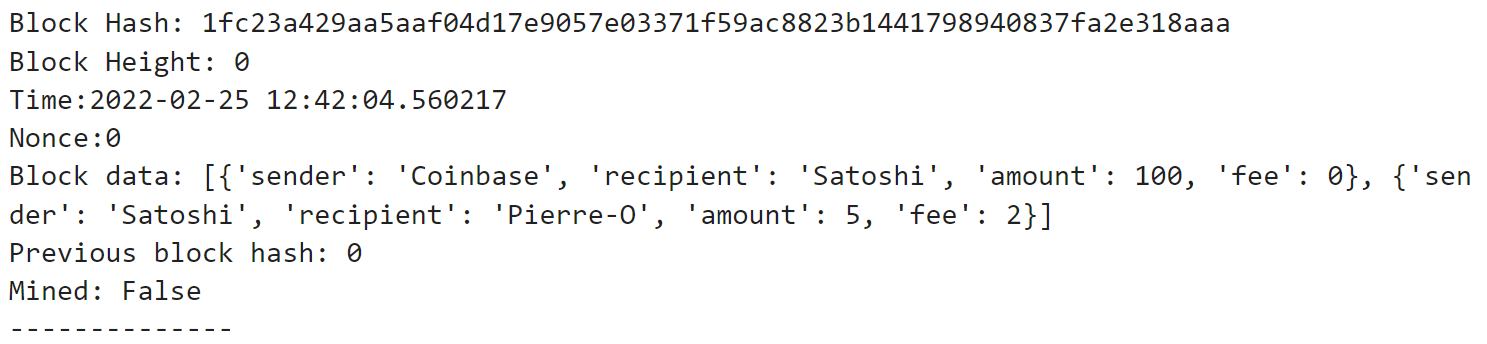
\includegraphics[width = \textwidth]{../../../Figures/block_not_mined.png}
    \captionsetup{width=0.8\textwidth}
    \centering
    \caption{A block that has not been mined yet.}
    \label{fig:block_not_mined}
\end{figure}
\end{frame}
\begin{frame}{Mining a block}
The maximum value for a 256 bits number is
$$
T_\text{max} = 2^{256}-1 \approx 1.16e^{77}
$$
mining consists in drawing at random a nonce 
$$
\text{Nonce} \sim \text{Unif}(\{0,\ldots, 2^{32}-1\})
$$
until 
$$
h(\text{Nonce}|\text{Block info})<T,
$$
where $T$ is referred to as the target.
\begin{tcolorbox}[enhanced,drop shadow, title=Difficulty of the cryptopuzzle]
$$
D = \frac{T_{\max}}{T}
$$
\end{tcolorbox}

\end{frame}
\begin{frame}{Mining a block}
If we set the difficulty to $D = 2^4$ then the hexadecimal digest must start with at least $1$ leading $0$
\begin{figure}[!ht]
    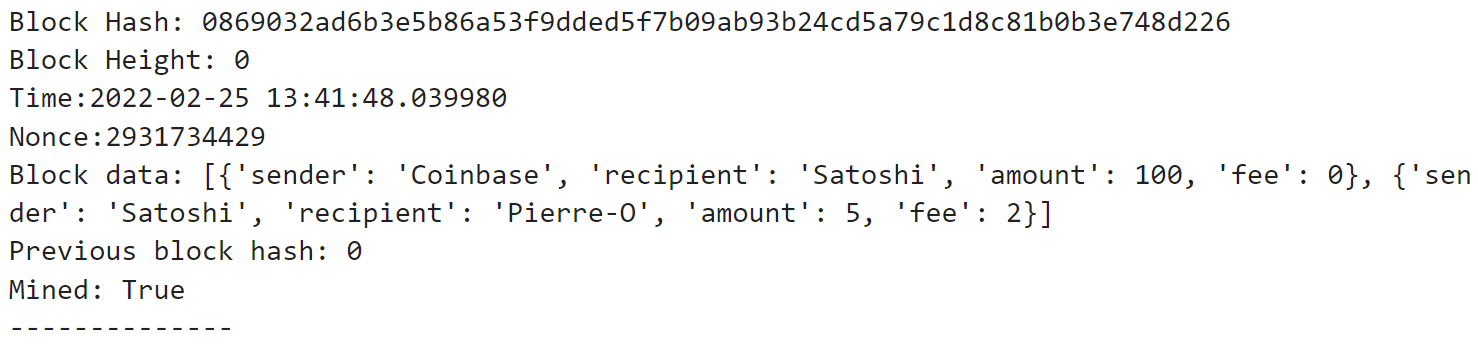
\includegraphics[width = \textwidth]{../../../Figures/block_mined.png}
    \captionsetup{width=0.8\textwidth}
    \centering
    \caption{A mined block with a hash value having on leading zero.}
    \label{fig:block_mined}
\end{figure}
The number of trial is geometrically distributed
\begin{itemize}
\item Exponential inter-block times
\item Lenght of the blockchain = Poisson process
\end{itemize}
\end{frame}
\begin{frame}{Bitcoin protocol}
\begin{itemize}
  \item One block every 10 minutes on average
  \item Depends on the hashrate of the network
  \item Difficulty adjustment every 2,016 blocks ($\approx$ two weeks)
  \item Reward halving every 210,000 blocks
\end{itemize}
Check out \url{https://www.bitcoinblockhalf.com/}
\end{frame}
\begin{frame}{Mining equipments}
How it started
\begin{itemize}
  \item CPU, GPU
\end{itemize}
How it is going
\begin{itemize}
  \item Application Specific Integrated Chip (ASIC)
  \begin{itemize}
  \item Increase of the network electricity consumption \url{https://digiconomist.net/bitcoin-energy-consumption}
  \item E-Waste
  \item Centralization issue \url{https://www.bitmain.com/}
  \begin{itemize}
    \item Mining pool ranking at \url{https://btc.com/}
    \item Mining equipment profitability at \url{https://v3.antpool.com/minerIncomeRank}
  \end{itemize}
  \end{itemize}
\end{itemize}
\end{frame}

\begin{frame}{Proof of Stake}
PoW is slow and ressource consuming. Let $\{1,\ldots, N\}$ be a set of miners and $\{\pi_1,\ldots, \pi_N\}$ be their share of cryptocoins.
\begin{tcolorbox}[enhanced,drop shadow, title=PoS]
\begin{enumerate}
\item Node $i\in \{1,\ldots, N\}$ is selected with probability $\pi_i$ to append the next block
\end{enumerate}
\end{tcolorbox}
\vspace{0.3cm}
Nodes are chosen according to what they own.
\begin{itemize}
  \item Nothing at stake problem
  \item Rich gets richer ? 
\end{itemize}
\footnotesize{
\begin{thebibliography}{1}

\bibitem{Saleh2020}
F.~Saleh, ``Blockchain without waste: Proof-of-stake,'' {\em The Review of
  Financial Studies}, vol.~34, pp.~1156--1190, jul 2020.

\end{thebibliography}}

\end{frame}


\end{document}
